% Created by tikzDevice version 0.10.1 on 2017-11-26 21:02:39
% !TEX encoding = UTF-8 Unicode
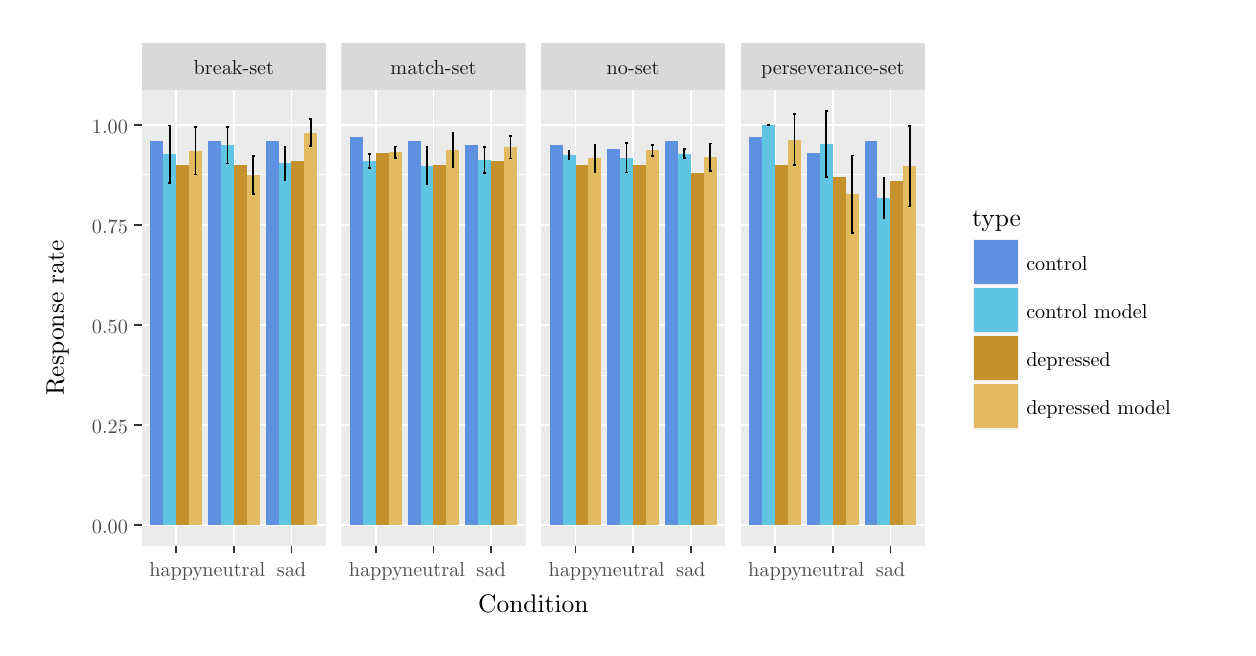
\begin{tikzpicture}[x=1pt,y=1pt]
\definecolor{fillColor}{RGB}{255,255,255}
\path[use as bounding box,fill=fillColor,fill opacity=0.00] (0,0) rectangle (433.62,216.81);
\begin{scope}
\path[clip] (  0.00,  0.00) rectangle (433.62,216.81);
\definecolor{drawColor}{RGB}{255,255,255}
\definecolor{fillColor}{RGB}{255,255,255}

\path[draw=drawColor,line width= 0.6pt,line join=round,line cap=round,fill=fillColor] (  0.00,  0.00) rectangle (433.62,216.81);
\end{scope}
\begin{scope}
\path[clip] ( 41.17, 29.59) rectangle (107.82,194.25);
\definecolor{fillColor}{gray}{0.92}

\path[fill=fillColor] ( 41.17, 29.59) rectangle (107.82,194.25);
\definecolor{drawColor}{RGB}{255,255,255}

\path[draw=drawColor,line width= 0.3pt,line join=round] ( 41.17, 55.15) --
	(107.82, 55.15);

\path[draw=drawColor,line width= 0.3pt,line join=round] ( 41.17, 91.32) --
	(107.82, 91.32);

\path[draw=drawColor,line width= 0.3pt,line join=round] ( 41.17,127.48) --
	(107.82,127.48);

\path[draw=drawColor,line width= 0.3pt,line join=round] ( 41.17,163.64) --
	(107.82,163.64);

\path[draw=drawColor,line width= 0.6pt,line join=round] ( 41.17, 37.07) --
	(107.82, 37.07);

\path[draw=drawColor,line width= 0.6pt,line join=round] ( 41.17, 73.23) --
	(107.82, 73.23);

\path[draw=drawColor,line width= 0.6pt,line join=round] ( 41.17,109.40) --
	(107.82,109.40);

\path[draw=drawColor,line width= 0.6pt,line join=round] ( 41.17,145.56) --
	(107.82,145.56);

\path[draw=drawColor,line width= 0.6pt,line join=round] ( 41.17,181.72) --
	(107.82,181.72);

\path[draw=drawColor,line width= 0.6pt,line join=round] ( 53.67, 29.59) --
	( 53.67,194.25);

\path[draw=drawColor,line width= 0.6pt,line join=round] ( 74.50, 29.59) --
	( 74.50,194.25);

\path[draw=drawColor,line width= 0.6pt,line join=round] ( 95.32, 29.59) --
	( 95.32,194.25);
\definecolor{fillColor}{RGB}{226,186,95}

\path[fill=fillColor] ( 58.36, 37.07) rectangle ( 63.04,172.34);
\definecolor{fillColor}{RGB}{196,145,45}

\path[fill=fillColor] ( 53.67, 37.07) rectangle ( 58.36,167.26);
\definecolor{fillColor}{RGB}{95,197,226}

\path[fill=fillColor] ( 48.98, 37.07) rectangle ( 53.67,171.13);
\definecolor{fillColor}{RGB}{95,145,226}

\path[fill=fillColor] ( 44.30, 37.07) rectangle ( 48.98,175.94);
\definecolor{fillColor}{RGB}{226,186,95}

\path[fill=fillColor] ( 79.18, 37.07) rectangle ( 83.87,163.52);
\definecolor{fillColor}{RGB}{196,145,45}

\path[fill=fillColor] ( 74.50, 37.07) rectangle ( 79.18,167.26);
\definecolor{fillColor}{RGB}{95,197,226}

\path[fill=fillColor] ( 69.81, 37.07) rectangle ( 74.50,174.32);
\definecolor{fillColor}{RGB}{95,145,226}

\path[fill=fillColor] ( 65.12, 37.07) rectangle ( 69.81,175.94);
\definecolor{fillColor}{RGB}{226,186,95}

\path[fill=fillColor] (100.01, 37.07) rectangle (104.69,178.89);
\definecolor{fillColor}{RGB}{196,145,45}

\path[fill=fillColor] ( 95.32, 37.07) rectangle (100.01,168.70);
\definecolor{fillColor}{RGB}{95,197,226}

\path[fill=fillColor] ( 90.64, 37.07) rectangle ( 95.32,167.80);
\definecolor{fillColor}{RGB}{95,145,226}

\path[fill=fillColor] ( 85.95, 37.07) rectangle ( 90.64,175.94);
\definecolor{drawColor}{RGB}{0,0,0}

\path[draw=drawColor,line width= 0.6pt,line join=round] ( 60.18,180.98) --
	( 61.22,180.98);

\path[draw=drawColor,line width= 0.6pt,line join=round] ( 60.70,180.98) --
	( 60.70,163.70);

\path[draw=drawColor,line width= 0.6pt,line join=round] ( 60.18,163.70) --
	( 61.22,163.70);

\path[draw=drawColor,line width= 0.6pt,line join=round] ( 50.81,181.47) --
	( 51.85,181.47);

\path[draw=drawColor,line width= 0.6pt,line join=round] ( 51.33,181.47) --
	( 51.33,160.78);

\path[draw=drawColor,line width= 0.6pt,line join=round] ( 50.81,160.78) --
	( 51.85,160.78);

\path[draw=drawColor,line width= 0.6pt,line join=round] ( 81.00,170.34) --
	( 82.05,170.34);

\path[draw=drawColor,line width= 0.6pt,line join=round] ( 81.52,170.34) --
	( 81.52,156.71);

\path[draw=drawColor,line width= 0.6pt,line join=round] ( 81.00,156.71) --
	( 82.05,156.71);

\path[draw=drawColor,line width= 0.6pt,line join=round] ( 71.63,180.90) --
	( 72.67,180.90);

\path[draw=drawColor,line width= 0.6pt,line join=round] ( 72.15,180.90) --
	( 72.15,167.73);

\path[draw=drawColor,line width= 0.6pt,line join=round] ( 71.63,167.73) --
	( 72.67,167.73);

\path[draw=drawColor,line width= 0.6pt,line join=round] (101.83,183.80) --
	(102.87,183.80);

\path[draw=drawColor,line width= 0.6pt,line join=round] (102.35,183.80) --
	(102.35,173.97);

\path[draw=drawColor,line width= 0.6pt,line join=round] (101.83,173.97) --
	(102.87,173.97);

\path[draw=drawColor,line width= 0.6pt,line join=round] ( 92.46,173.83) --
	( 93.50,173.83);

\path[draw=drawColor,line width= 0.6pt,line join=round] ( 92.98,173.83) --
	( 92.98,161.77);

\path[draw=drawColor,line width= 0.6pt,line join=round] ( 92.46,161.77) --
	( 93.50,161.77);
\end{scope}
\begin{scope}
\path[clip] (113.32, 29.59) rectangle (179.96,194.25);
\definecolor{fillColor}{gray}{0.92}

\path[fill=fillColor] (113.32, 29.59) rectangle (179.96,194.25);
\definecolor{drawColor}{RGB}{255,255,255}

\path[draw=drawColor,line width= 0.3pt,line join=round] (113.32, 55.15) --
	(179.96, 55.15);

\path[draw=drawColor,line width= 0.3pt,line join=round] (113.32, 91.32) --
	(179.96, 91.32);

\path[draw=drawColor,line width= 0.3pt,line join=round] (113.32,127.48) --
	(179.96,127.48);

\path[draw=drawColor,line width= 0.3pt,line join=round] (113.32,163.64) --
	(179.96,163.64);

\path[draw=drawColor,line width= 0.6pt,line join=round] (113.32, 37.07) --
	(179.96, 37.07);

\path[draw=drawColor,line width= 0.6pt,line join=round] (113.32, 73.23) --
	(179.96, 73.23);

\path[draw=drawColor,line width= 0.6pt,line join=round] (113.32,109.40) --
	(179.96,109.40);

\path[draw=drawColor,line width= 0.6pt,line join=round] (113.32,145.56) --
	(179.96,145.56);

\path[draw=drawColor,line width= 0.6pt,line join=round] (113.32,181.72) --
	(179.96,181.72);

\path[draw=drawColor,line width= 0.6pt,line join=round] (125.81, 29.59) --
	(125.81,194.25);

\path[draw=drawColor,line width= 0.6pt,line join=round] (146.64, 29.59) --
	(146.64,194.25);

\path[draw=drawColor,line width= 0.6pt,line join=round] (167.47, 29.59) --
	(167.47,194.25);
\definecolor{fillColor}{RGB}{226,186,95}

\path[fill=fillColor] (130.50, 37.07) rectangle (135.19,171.81);
\definecolor{fillColor}{RGB}{196,145,45}

\path[fill=fillColor] (125.81, 37.07) rectangle (130.50,171.60);
\definecolor{fillColor}{RGB}{95,197,226}

\path[fill=fillColor] (121.13, 37.07) rectangle (125.81,168.65);
\definecolor{fillColor}{RGB}{95,145,226}

\path[fill=fillColor] (116.44, 37.07) rectangle (121.13,177.38);
\definecolor{fillColor}{RGB}{226,186,95}

\path[fill=fillColor] (151.33, 37.07) rectangle (156.01,172.57);
\definecolor{fillColor}{RGB}{196,145,45}

\path[fill=fillColor] (146.64, 37.07) rectangle (151.33,167.26);
\definecolor{fillColor}{RGB}{95,197,226}

\path[fill=fillColor] (141.95, 37.07) rectangle (146.64,166.95);
\definecolor{fillColor}{RGB}{95,145,226}

\path[fill=fillColor] (137.27, 37.07) rectangle (141.95,175.94);
\definecolor{fillColor}{RGB}{226,186,95}

\path[fill=fillColor] (172.15, 37.07) rectangle (176.84,173.53);
\definecolor{fillColor}{RGB}{196,145,45}

\path[fill=fillColor] (167.47, 37.07) rectangle (172.15,168.70);
\definecolor{fillColor}{RGB}{95,197,226}

\path[fill=fillColor] (162.78, 37.07) rectangle (167.47,168.97);
\definecolor{fillColor}{RGB}{95,145,226}

\path[fill=fillColor] (158.10, 37.07) rectangle (162.78,174.49);
\definecolor{drawColor}{RGB}{0,0,0}

\path[draw=drawColor,line width= 0.6pt,line join=round] (132.32,173.83) --
	(133.36,173.83);

\path[draw=drawColor,line width= 0.6pt,line join=round] (132.84,173.83) --
	(132.84,169.79);

\path[draw=drawColor,line width= 0.6pt,line join=round] (132.32,169.79) --
	(133.36,169.79);

\path[draw=drawColor,line width= 0.6pt,line join=round] (122.95,171.25) --
	(123.99,171.25);

\path[draw=drawColor,line width= 0.6pt,line join=round] (123.47,171.25) --
	(123.47,166.05);

\path[draw=drawColor,line width= 0.6pt,line join=round] (122.95,166.05) --
	(123.99,166.05);

\path[draw=drawColor,line width= 0.6pt,line join=round] (153.15,178.65) --
	(154.19,178.65);

\path[draw=drawColor,line width= 0.6pt,line join=round] (153.67,178.65) --
	(153.67,166.49);

\path[draw=drawColor,line width= 0.6pt,line join=round] (153.15,166.49) --
	(154.19,166.49);

\path[draw=drawColor,line width= 0.6pt,line join=round] (143.78,173.79) --
	(144.82,173.79);

\path[draw=drawColor,line width= 0.6pt,line join=round] (144.30,173.79) --
	(144.30,160.11);

\path[draw=drawColor,line width= 0.6pt,line join=round] (143.78,160.11) --
	(144.82,160.11);

\path[draw=drawColor,line width= 0.6pt,line join=round] (173.98,177.56) --
	(175.02,177.56);

\path[draw=drawColor,line width= 0.6pt,line join=round] (174.50,177.56) --
	(174.50,169.50);

\path[draw=drawColor,line width= 0.6pt,line join=round] (173.98,169.50) --
	(175.02,169.50);

\path[draw=drawColor,line width= 0.6pt,line join=round] (164.60,173.58) --
	(165.64,173.58);

\path[draw=drawColor,line width= 0.6pt,line join=round] (165.12,173.58) --
	(165.12,164.36);

\path[draw=drawColor,line width= 0.6pt,line join=round] (164.60,164.36) --
	(165.64,164.36);
\end{scope}
\begin{scope}
\path[clip] (185.46, 29.59) rectangle (252.11,194.25);
\definecolor{fillColor}{gray}{0.92}

\path[fill=fillColor] (185.46, 29.59) rectangle (252.11,194.25);
\definecolor{drawColor}{RGB}{255,255,255}

\path[draw=drawColor,line width= 0.3pt,line join=round] (185.46, 55.15) --
	(252.11, 55.15);

\path[draw=drawColor,line width= 0.3pt,line join=round] (185.46, 91.32) --
	(252.11, 91.32);

\path[draw=drawColor,line width= 0.3pt,line join=round] (185.46,127.48) --
	(252.11,127.48);

\path[draw=drawColor,line width= 0.3pt,line join=round] (185.46,163.64) --
	(252.11,163.64);

\path[draw=drawColor,line width= 0.6pt,line join=round] (185.46, 37.07) --
	(252.11, 37.07);

\path[draw=drawColor,line width= 0.6pt,line join=round] (185.46, 73.23) --
	(252.11, 73.23);

\path[draw=drawColor,line width= 0.6pt,line join=round] (185.46,109.40) --
	(252.11,109.40);

\path[draw=drawColor,line width= 0.6pt,line join=round] (185.46,145.56) --
	(252.11,145.56);

\path[draw=drawColor,line width= 0.6pt,line join=round] (185.46,181.72) --
	(252.11,181.72);

\path[draw=drawColor,line width= 0.6pt,line join=round] (197.96, 29.59) --
	(197.96,194.25);

\path[draw=drawColor,line width= 0.6pt,line join=round] (218.79, 29.59) --
	(218.79,194.25);

\path[draw=drawColor,line width= 0.6pt,line join=round] (239.61, 29.59) --
	(239.61,194.25);
\definecolor{fillColor}{RGB}{226,186,95}

\path[fill=fillColor] (202.64, 37.07) rectangle (207.33,169.64);
\definecolor{fillColor}{RGB}{196,145,45}

\path[fill=fillColor] (197.96, 37.07) rectangle (202.64,167.26);
\definecolor{fillColor}{RGB}{95,197,226}

\path[fill=fillColor] (193.27, 37.07) rectangle (197.96,170.78);
\definecolor{fillColor}{RGB}{95,145,226}

\path[fill=fillColor] (188.59, 37.07) rectangle (193.27,174.49);
\definecolor{fillColor}{RGB}{226,186,95}

\path[fill=fillColor] (223.47, 37.07) rectangle (228.16,172.54);
\definecolor{fillColor}{RGB}{196,145,45}

\path[fill=fillColor] (218.79, 37.07) rectangle (223.47,167.26);
\definecolor{fillColor}{RGB}{95,197,226}

\path[fill=fillColor] (214.10, 37.07) rectangle (218.79,169.82);
\definecolor{fillColor}{RGB}{95,145,226}

\path[fill=fillColor] (209.41, 37.07) rectangle (214.10,173.04);
\definecolor{fillColor}{RGB}{226,186,95}

\path[fill=fillColor] (244.30, 37.07) rectangle (248.98,169.97);
\definecolor{fillColor}{RGB}{196,145,45}

\path[fill=fillColor] (239.61, 37.07) rectangle (244.30,164.36);
\definecolor{fillColor}{RGB}{95,197,226}

\path[fill=fillColor] (234.93, 37.07) rectangle (239.61,171.26);
\definecolor{fillColor}{RGB}{95,145,226}

\path[fill=fillColor] (230.24, 37.07) rectangle (234.93,175.94);
\definecolor{drawColor}{RGB}{0,0,0}

\path[draw=drawColor,line width= 0.6pt,line join=round] (204.47,174.57) --
	(205.51,174.57);

\path[draw=drawColor,line width= 0.6pt,line join=round] (204.99,174.57) --
	(204.99,164.72);

\path[draw=drawColor,line width= 0.6pt,line join=round] (204.47,164.72) --
	(205.51,164.72);

\path[draw=drawColor,line width= 0.6pt,line join=round] (195.10,172.13) --
	(196.14,172.13);

\path[draw=drawColor,line width= 0.6pt,line join=round] (195.62,172.13) --
	(195.62,169.42);

\path[draw=drawColor,line width= 0.6pt,line join=round] (195.10,169.42) --
	(196.14,169.42);

\path[draw=drawColor,line width= 0.6pt,line join=round] (225.29,174.53) --
	(226.34,174.53);

\path[draw=drawColor,line width= 0.6pt,line join=round] (225.81,174.53) --
	(225.81,170.55);

\path[draw=drawColor,line width= 0.6pt,line join=round] (225.29,170.55) --
	(226.34,170.55);

\path[draw=drawColor,line width= 0.6pt,line join=round] (215.92,175.21) --
	(216.96,175.21);

\path[draw=drawColor,line width= 0.6pt,line join=round] (216.44,175.21) --
	(216.44,164.43);

\path[draw=drawColor,line width= 0.6pt,line join=round] (215.92,164.43) --
	(216.96,164.43);

\path[draw=drawColor,line width= 0.6pt,line join=round] (246.12,174.93) --
	(247.16,174.93);

\path[draw=drawColor,line width= 0.6pt,line join=round] (246.64,174.93) --
	(246.64,165.01);

\path[draw=drawColor,line width= 0.6pt,line join=round] (246.12,165.01) --
	(247.16,165.01);

\path[draw=drawColor,line width= 0.6pt,line join=round] (236.75,172.86) --
	(237.79,172.86);

\path[draw=drawColor,line width= 0.6pt,line join=round] (237.27,172.86) --
	(237.27,169.66);

\path[draw=drawColor,line width= 0.6pt,line join=round] (236.75,169.66) --
	(237.79,169.66);
\end{scope}
\begin{scope}
\path[clip] (257.61, 29.59) rectangle (324.25,194.25);
\definecolor{fillColor}{gray}{0.92}

\path[fill=fillColor] (257.61, 29.59) rectangle (324.25,194.25);
\definecolor{drawColor}{RGB}{255,255,255}

\path[draw=drawColor,line width= 0.3pt,line join=round] (257.61, 55.15) --
	(324.25, 55.15);

\path[draw=drawColor,line width= 0.3pt,line join=round] (257.61, 91.32) --
	(324.25, 91.32);

\path[draw=drawColor,line width= 0.3pt,line join=round] (257.61,127.48) --
	(324.25,127.48);

\path[draw=drawColor,line width= 0.3pt,line join=round] (257.61,163.64) --
	(324.25,163.64);

\path[draw=drawColor,line width= 0.6pt,line join=round] (257.61, 37.07) --
	(324.25, 37.07);

\path[draw=drawColor,line width= 0.6pt,line join=round] (257.61, 73.23) --
	(324.25, 73.23);

\path[draw=drawColor,line width= 0.6pt,line join=round] (257.61,109.40) --
	(324.25,109.40);

\path[draw=drawColor,line width= 0.6pt,line join=round] (257.61,145.56) --
	(324.25,145.56);

\path[draw=drawColor,line width= 0.6pt,line join=round] (257.61,181.72) --
	(324.25,181.72);

\path[draw=drawColor,line width= 0.6pt,line join=round] (270.10, 29.59) --
	(270.10,194.25);

\path[draw=drawColor,line width= 0.6pt,line join=round] (290.93, 29.59) --
	(290.93,194.25);

\path[draw=drawColor,line width= 0.6pt,line join=round] (311.76, 29.59) --
	(311.76,194.25);
\definecolor{fillColor}{RGB}{226,186,95}

\path[fill=fillColor] (274.79, 37.07) rectangle (279.48,176.36);
\definecolor{fillColor}{RGB}{196,145,45}

\path[fill=fillColor] (270.10, 37.07) rectangle (274.79,167.26);
\definecolor{fillColor}{RGB}{95,197,226}

\path[fill=fillColor] (265.42, 37.07) rectangle (270.10,181.72);
\definecolor{fillColor}{RGB}{95,145,226}

\path[fill=fillColor] (260.73, 37.07) rectangle (265.42,177.38);
\definecolor{fillColor}{RGB}{226,186,95}

\path[fill=fillColor] (295.62, 37.07) rectangle (300.30,156.56);
\definecolor{fillColor}{RGB}{196,145,45}

\path[fill=fillColor] (290.93, 37.07) rectangle (295.62,162.92);
\definecolor{fillColor}{RGB}{95,197,226}

\path[fill=fillColor] (286.24, 37.07) rectangle (290.93,174.83);
\definecolor{fillColor}{RGB}{95,145,226}

\path[fill=fillColor] (281.56, 37.07) rectangle (286.24,171.60);
\definecolor{fillColor}{RGB}{226,186,95}

\path[fill=fillColor] (316.44, 37.07) rectangle (321.13,166.72);
\definecolor{fillColor}{RGB}{196,145,45}

\path[fill=fillColor] (311.76, 37.07) rectangle (316.44,161.47);
\definecolor{fillColor}{RGB}{95,197,226}

\path[fill=fillColor] (307.07, 37.07) rectangle (311.76,155.34);
\definecolor{fillColor}{RGB}{95,145,226}

\path[fill=fillColor] (302.39, 37.07) rectangle (307.07,175.94);
\definecolor{drawColor}{RGB}{0,0,0}

\path[draw=drawColor,line width= 0.6pt,line join=round] (276.61,185.64) --
	(277.65,185.64);

\path[draw=drawColor,line width= 0.6pt,line join=round] (277.13,185.64) --
	(277.13,167.09);

\path[draw=drawColor,line width= 0.6pt,line join=round] (276.61,167.09) --
	(277.65,167.09);

\path[draw=drawColor,line width= 0.6pt,line join=round] (267.24,181.72) --
	(268.28,181.72);

\path[draw=drawColor,line width= 0.6pt,line join=round] (267.76,181.72) --
	(267.76,181.72);

\path[draw=drawColor,line width= 0.6pt,line join=round] (267.24,181.72) --
	(268.28,181.72);

\path[draw=drawColor,line width= 0.6pt,line join=round] (297.44,170.60) --
	(298.48,170.60);

\path[draw=drawColor,line width= 0.6pt,line join=round] (297.96,170.60) --
	(297.96,142.52);

\path[draw=drawColor,line width= 0.6pt,line join=round] (297.44,142.52) --
	(298.48,142.52);

\path[draw=drawColor,line width= 0.6pt,line join=round] (288.07,186.76) --
	(289.11,186.76);

\path[draw=drawColor,line width= 0.6pt,line join=round] (288.59,186.76) --
	(288.59,162.90);

\path[draw=drawColor,line width= 0.6pt,line join=round] (288.07,162.90) --
	(289.11,162.90);

\path[draw=drawColor,line width= 0.6pt,line join=round] (318.27,181.22) --
	(319.31,181.22);

\path[draw=drawColor,line width= 0.6pt,line join=round] (318.79,181.22) --
	(318.79,152.23);

\path[draw=drawColor,line width= 0.6pt,line join=round] (318.27,152.23) --
	(319.31,152.23);

\path[draw=drawColor,line width= 0.6pt,line join=round] (308.89,162.71) --
	(309.93,162.71);

\path[draw=drawColor,line width= 0.6pt,line join=round] (309.41,162.71) --
	(309.41,147.97);

\path[draw=drawColor,line width= 0.6pt,line join=round] (308.89,147.97) --
	(309.93,147.97);
\end{scope}
\begin{scope}
\path[clip] ( 41.17,194.25) rectangle (107.82,211.31);
\definecolor{fillColor}{gray}{0.85}

\path[fill=fillColor] ( 41.17,194.25) rectangle (107.82,211.31);
\definecolor{drawColor}{gray}{0.10}

\node[text=drawColor,anchor=base,inner sep=0pt, outer sep=0pt, scale=  0.73] at ( 74.50,199.75) {break-set};
\end{scope}
\begin{scope}
\path[clip] (113.32,194.25) rectangle (179.96,211.31);
\definecolor{fillColor}{gray}{0.85}

\path[fill=fillColor] (113.32,194.25) rectangle (179.96,211.31);
\definecolor{drawColor}{gray}{0.10}

\node[text=drawColor,anchor=base,inner sep=0pt, outer sep=0pt, scale=  0.73] at (146.64,199.75) {match-set};
\end{scope}
\begin{scope}
\path[clip] (185.46,194.25) rectangle (252.11,211.31);
\definecolor{fillColor}{gray}{0.85}

\path[fill=fillColor] (185.46,194.25) rectangle (252.11,211.31);
\definecolor{drawColor}{gray}{0.10}

\node[text=drawColor,anchor=base,inner sep=0pt, outer sep=0pt, scale=  0.73] at (218.79,199.75) {no-set};
\end{scope}
\begin{scope}
\path[clip] (257.61,194.25) rectangle (324.25,211.31);
\definecolor{fillColor}{gray}{0.85}

\path[fill=fillColor] (257.61,194.25) rectangle (324.25,211.31);
\definecolor{drawColor}{gray}{0.10}

\node[text=drawColor,anchor=base,inner sep=0pt, outer sep=0pt, scale=  0.73] at (290.93,199.75) {perseverance-set};
\end{scope}
\begin{scope}
\path[clip] (  0.00,  0.00) rectangle (433.62,216.81);
\definecolor{drawColor}{gray}{0.20}

\path[draw=drawColor,line width= 0.6pt,line join=round] ( 53.67, 26.84) --
	( 53.67, 29.59);

\path[draw=drawColor,line width= 0.6pt,line join=round] ( 74.50, 26.84) --
	( 74.50, 29.59);

\path[draw=drawColor,line width= 0.6pt,line join=round] ( 95.32, 26.84) --
	( 95.32, 29.59);
\end{scope}
\begin{scope}
\path[clip] (  0.00,  0.00) rectangle (433.62,216.81);
\definecolor{drawColor}{gray}{0.30}

\node[text=drawColor,anchor=base,inner sep=0pt, outer sep=0pt, scale=  0.73] at ( 53.67, 18.58) {happy};

\node[text=drawColor,anchor=base,inner sep=0pt, outer sep=0pt, scale=  0.73] at ( 74.50, 18.58) {neutral};

\node[text=drawColor,anchor=base,inner sep=0pt, outer sep=0pt, scale=  0.73] at ( 95.32, 18.58) {sad};
\end{scope}
\begin{scope}
\path[clip] (  0.00,  0.00) rectangle (433.62,216.81);
\definecolor{drawColor}{gray}{0.20}

\path[draw=drawColor,line width= 0.6pt,line join=round] (125.81, 26.84) --
	(125.81, 29.59);

\path[draw=drawColor,line width= 0.6pt,line join=round] (146.64, 26.84) --
	(146.64, 29.59);

\path[draw=drawColor,line width= 0.6pt,line join=round] (167.47, 26.84) --
	(167.47, 29.59);
\end{scope}
\begin{scope}
\path[clip] (  0.00,  0.00) rectangle (433.62,216.81);
\definecolor{drawColor}{gray}{0.30}

\node[text=drawColor,anchor=base,inner sep=0pt, outer sep=0pt, scale=  0.73] at (125.81, 18.58) {happy};

\node[text=drawColor,anchor=base,inner sep=0pt, outer sep=0pt, scale=  0.73] at (146.64, 18.58) {neutral};

\node[text=drawColor,anchor=base,inner sep=0pt, outer sep=0pt, scale=  0.73] at (167.47, 18.58) {sad};
\end{scope}
\begin{scope}
\path[clip] (  0.00,  0.00) rectangle (433.62,216.81);
\definecolor{drawColor}{gray}{0.20}

\path[draw=drawColor,line width= 0.6pt,line join=round] (197.96, 26.84) --
	(197.96, 29.59);

\path[draw=drawColor,line width= 0.6pt,line join=round] (218.79, 26.84) --
	(218.79, 29.59);

\path[draw=drawColor,line width= 0.6pt,line join=round] (239.61, 26.84) --
	(239.61, 29.59);
\end{scope}
\begin{scope}
\path[clip] (  0.00,  0.00) rectangle (433.62,216.81);
\definecolor{drawColor}{gray}{0.30}

\node[text=drawColor,anchor=base,inner sep=0pt, outer sep=0pt, scale=  0.73] at (197.96, 18.58) {happy};

\node[text=drawColor,anchor=base,inner sep=0pt, outer sep=0pt, scale=  0.73] at (218.79, 18.58) {neutral};

\node[text=drawColor,anchor=base,inner sep=0pt, outer sep=0pt, scale=  0.73] at (239.61, 18.58) {sad};
\end{scope}
\begin{scope}
\path[clip] (  0.00,  0.00) rectangle (433.62,216.81);
\definecolor{drawColor}{gray}{0.20}

\path[draw=drawColor,line width= 0.6pt,line join=round] (270.10, 26.84) --
	(270.10, 29.59);

\path[draw=drawColor,line width= 0.6pt,line join=round] (290.93, 26.84) --
	(290.93, 29.59);

\path[draw=drawColor,line width= 0.6pt,line join=round] (311.76, 26.84) --
	(311.76, 29.59);
\end{scope}
\begin{scope}
\path[clip] (  0.00,  0.00) rectangle (433.62,216.81);
\definecolor{drawColor}{gray}{0.30}

\node[text=drawColor,anchor=base,inner sep=0pt, outer sep=0pt, scale=  0.73] at (270.10, 18.58) {happy};

\node[text=drawColor,anchor=base,inner sep=0pt, outer sep=0pt, scale=  0.73] at (290.93, 18.58) {neutral};

\node[text=drawColor,anchor=base,inner sep=0pt, outer sep=0pt, scale=  0.73] at (311.76, 18.58) {sad};
\end{scope}
\begin{scope}
\path[clip] (  0.00,  0.00) rectangle (433.62,216.81);
\definecolor{drawColor}{gray}{0.30}

\node[text=drawColor,anchor=base east,inner sep=0pt, outer sep=0pt, scale=  0.73] at ( 36.22, 34.04) {0.00};

\node[text=drawColor,anchor=base east,inner sep=0pt, outer sep=0pt, scale=  0.73] at ( 36.22, 70.20) {0.25};

\node[text=drawColor,anchor=base east,inner sep=0pt, outer sep=0pt, scale=  0.73] at ( 36.22,106.37) {0.50};

\node[text=drawColor,anchor=base east,inner sep=0pt, outer sep=0pt, scale=  0.73] at ( 36.22,142.53) {0.75};

\node[text=drawColor,anchor=base east,inner sep=0pt, outer sep=0pt, scale=  0.73] at ( 36.22,178.69) {1.00};
\end{scope}
\begin{scope}
\path[clip] (  0.00,  0.00) rectangle (433.62,216.81);
\definecolor{drawColor}{gray}{0.20}

\path[draw=drawColor,line width= 0.6pt,line join=round] ( 38.42, 37.07) --
	( 41.17, 37.07);

\path[draw=drawColor,line width= 0.6pt,line join=round] ( 38.42, 73.23) --
	( 41.17, 73.23);

\path[draw=drawColor,line width= 0.6pt,line join=round] ( 38.42,109.40) --
	( 41.17,109.40);

\path[draw=drawColor,line width= 0.6pt,line join=round] ( 38.42,145.56) --
	( 41.17,145.56);

\path[draw=drawColor,line width= 0.6pt,line join=round] ( 38.42,181.72) --
	( 41.17,181.72);
\end{scope}
\begin{scope}
\path[clip] (  0.00,  0.00) rectangle (433.62,216.81);
\definecolor{drawColor}{RGB}{0,0,0}

\node[text=drawColor,anchor=base,inner sep=0pt, outer sep=0pt, scale=  0.92] at (182.71,  5.50) {Condition};
\end{scope}
\begin{scope}
\path[clip] (  0.00,  0.00) rectangle (433.62,216.81);
\definecolor{drawColor}{RGB}{0,0,0}

\node[text=drawColor,rotate= 90.00,anchor=base,inner sep=0pt, outer sep=0pt, scale=  0.92] at ( 13.08,111.92) {Response rate};
\end{scope}
\begin{scope}
\path[clip] (  0.00,  0.00) rectangle (433.62,216.81);
\definecolor{fillColor}{RGB}{255,255,255}

\path[fill=fillColor] (335.63, 65.58) rectangle (428.12,158.25);
\end{scope}
\begin{scope}
\path[clip] (  0.00,  0.00) rectangle (433.62,216.81);
\definecolor{drawColor}{RGB}{0,0,0}

\node[text=drawColor,anchor=base west,inner sep=0pt, outer sep=0pt, scale=  0.92] at (341.32,144.99) {type};
\end{scope}
\begin{scope}
\path[clip] (  0.00,  0.00) rectangle (433.62,216.81);
\definecolor{drawColor}{RGB}{255,255,255}
\definecolor{fillColor}{gray}{0.95}

\path[draw=drawColor,line width= 0.6pt,line join=round,line cap=round,fill=fillColor] (341.32,123.31) rectangle (358.67,140.65);
\end{scope}
\begin{scope}
\path[clip] (  0.00,  0.00) rectangle (433.62,216.81);
\definecolor{fillColor}{RGB}{95,145,226}

\path[fill=fillColor] (342.04,124.02) rectangle (357.96,139.94);
\end{scope}
\begin{scope}
\path[clip] (  0.00,  0.00) rectangle (433.62,216.81);
\definecolor{drawColor}{RGB}{255,255,255}
\definecolor{fillColor}{gray}{0.95}

\path[draw=drawColor,line width= 0.6pt,line join=round,line cap=round,fill=fillColor] (341.32,105.96) rectangle (358.67,123.31);
\end{scope}
\begin{scope}
\path[clip] (  0.00,  0.00) rectangle (433.62,216.81);
\definecolor{fillColor}{RGB}{95,197,226}

\path[fill=fillColor] (342.04,106.67) rectangle (357.96,122.60);
\end{scope}
\begin{scope}
\path[clip] (  0.00,  0.00) rectangle (433.62,216.81);
\definecolor{drawColor}{RGB}{255,255,255}
\definecolor{fillColor}{gray}{0.95}

\path[draw=drawColor,line width= 0.6pt,line join=round,line cap=round,fill=fillColor] (341.32, 88.62) rectangle (358.67,105.96);
\end{scope}
\begin{scope}
\path[clip] (  0.00,  0.00) rectangle (433.62,216.81);
\definecolor{fillColor}{RGB}{196,145,45}

\path[fill=fillColor] (342.04, 89.33) rectangle (357.96,105.25);
\end{scope}
\begin{scope}
\path[clip] (  0.00,  0.00) rectangle (433.62,216.81);
\definecolor{drawColor}{RGB}{255,255,255}
\definecolor{fillColor}{gray}{0.95}

\path[draw=drawColor,line width= 0.6pt,line join=round,line cap=round,fill=fillColor] (341.32, 71.27) rectangle (358.67, 88.62);
\end{scope}
\begin{scope}
\path[clip] (  0.00,  0.00) rectangle (433.62,216.81);
\definecolor{fillColor}{RGB}{226,186,95}

\path[fill=fillColor] (342.04, 71.98) rectangle (357.96, 87.91);
\end{scope}
\begin{scope}
\path[clip] (  0.00,  0.00) rectangle (433.62,216.81);
\definecolor{drawColor}{RGB}{0,0,0}

\node[text=drawColor,anchor=base west,inner sep=0pt, outer sep=0pt, scale=  0.73] at (360.84,128.95) {control};
\end{scope}
\begin{scope}
\path[clip] (  0.00,  0.00) rectangle (433.62,216.81);
\definecolor{drawColor}{RGB}{0,0,0}

\node[text=drawColor,anchor=base west,inner sep=0pt, outer sep=0pt, scale=  0.73] at (360.84,111.60) {control model};
\end{scope}
\begin{scope}
\path[clip] (  0.00,  0.00) rectangle (433.62,216.81);
\definecolor{drawColor}{RGB}{0,0,0}

\node[text=drawColor,anchor=base west,inner sep=0pt, outer sep=0pt, scale=  0.73] at (360.84, 94.26) {depressed};
\end{scope}
\begin{scope}
\path[clip] (  0.00,  0.00) rectangle (433.62,216.81);
\definecolor{drawColor}{RGB}{0,0,0}

\node[text=drawColor,anchor=base west,inner sep=0pt, outer sep=0pt, scale=  0.73] at (360.84, 76.91) {depressed model};
\end{scope}
\end{tikzpicture}
